\chapter{Analýza předchozí práce}\label{ch:analysis}



Daná diplomová práce navazuje na bakalářské práci z roku 2019~\cite{bachelorthesis} a využívá jak analýzu/výsledky popsané v práci samotné, tak i přílohy (zejména zdrojový kód serverové aplikace, klientské aplikace a vývojářské a uživatelské dokumentace).
Pro zajištění kvality výsledného \gls{IS} je provedena opakovaná analýza problematiky a korekce potřebných oblastí.



\section{Definované možnosti rozvoje a slabé stránky}



\subsection{Posudky}
Ze závěrečných posudků vedoucího a oponenta bakalářské práce je nutno vyčlenit několik významných bodů pro zlepšení.

\begin{ul}
   \item
   \textbf{Neúplná či nedostatečně propracovaná dokumentace~\cite{bachelorthesisreportsupervisor}} - je třeba přepracovat poskytnou informaci a doplnit relevantními informacemi.
   \item
   \textbf{Velice stručně popsané testování~\cite{bachelorthesisreportreviewer}} - v poskytnutém systému je velice málo automatizovaných testů a probíhalo zejména manuální testování~\cite{bachelorthesis} \TODO{paragraph cite}.
   \item
   \textbf{Nebylo popsané konkrétní určení informačního systému~\cite{bachelorthesisreportreviewer}} - informační systém od začátku nebyl cílený pro konkrétního spotřebitele.
   V dané práci bude celý informační systém brán pouze jako prostředek pro dosažení cíle práce.
\end{ul}

Zároveň během obhajoby bakalářské práce bylo nabídnuto zvážit vedení projektu ve \gls{VCS} git místo manuálního ukládání v NoSQL databázi (MongoDB).
To by jistým způsobem zredukovalo potřebného kódu a snížilo spotřebu paměti (jednotlivé snímky odevzdaných projektů by se neduplikovaly, ale ukládaly jako git značky).



\subsection{Možnosti rozvoje}

Bakalářská práce navrhuje rozvoj 2 hlavními směry - obecné univerzální zdokonalování a rozvoj se zaměřením na \gls{FIT} \gls{ČVUT}~\cite{bachelorthesis} \TODO{paragraph cite}.
Jelikož daná práce se soustředí především na \gls{MSA}, tak rozvoj se zaměřením na fakultu bude považován za sekundární.
V předchozí práci bylo nabídnuto několik bodů pro rozvoj~\cite{bachelorthesis} \TODO{paragraph cite}.


\begin{ul}
   \item
   \textbf{Podpora internacionalizace a lokalizace} - aplikace poskytuje pouze rozhraní v angličtině.
   Nepoužívá se žádný framework nebo knihovna, která by napomáhala snadné správě překladů.
   \item
   \textbf{Hromadné zakládání projektů} - neexistuje způsob hromadného zakládání projektů, i když dle předchozí analýzy by byl prospěšný.
   \item
   \textbf{Serverová implementace snímků} - nedokončená funkcionalita pro odevzdávání jednotlivých iterací projektů.
   \item
   \textbf{Nepříznivé scénáře \gls{API} dotazů} - v případě pádu serveru a neočekávané \gls{API} odpovědi často chybí uživatelsky přijatelné oznámení/zpracování.
   \item
   \textbf{Nové interprety obsahu} - jedná se o omezený výběr vytvářených typů obsahů.
   V dané práci není prioritní.
   \item
   \textbf{Propracovaná integrace se službami třetích stran} - daná funkcionalita se dotkne \gls{MSA}, rovněž není prioritní.
   \item
   \textbf{Analýza využití systému a aktualizace \gls{UX}} - bez produkčního prostředí (nebo jiného dlouhodobého uživatelského testování) nebylo možné získat daná data.
   \item
   \textbf{Optimalizace stávajícího systému} - různorodá optimalizace systému bude předmětem přechodu na \gls{MSA} a níže uvedené detailní revizí kódu.
\end{ul}

Všechny výše uvedené body pro rozvoj z původní práce~\cite{bachelorthesis} budou zváženy a případně vyřešeny v nové specifikaci projektu.



\subsection{Revize kódu}

\begin{ul}
   \item
   \textbf{\gls{IS} není plně kontejnerizovaný} - \gls{IS} není plně převeden na kontejnery, může být zdlouhavější start projektu, to se v pozdějších fázích odrazí i na předpokládané škálovatelnosti služby.
   \item
   \textbf{Monolitická struktura aplikace} - jakákoliv úprava vyžaduje editaci celého systému, není možné pohodlně měnit jednotlivé části aplikace.
   \item
   \textbf{Staré a vyřazené z provozu knihovny} - v klientské React aplikaci se nachází starší knihovny, jež musí být aktualizovány (bezpečnost, nová funkcionalita apod.).
   Rovněž je možné uplatnit nové způsoby psaní React aplikací (React Hooks \TODO{citace}).
   \item
   \textbf{Konfigurace a zbytečné oddělování prostředí} - bude potřeba zvážit konfiguraci přes \texttt{.env} soubory \TODO{citace} a odstranit rozdělení způsobů startu aplikace dle prostředí.
   \item
   \textbf{Struktura projektu, architektura} - některé prvky, struktura složek a návrh architektury se zdá být v některých případech zbytečný a přispívá nečitelnosti.
\end{ul}



\section{Silné stránky}
Z hlediska pozitivních prvků poskytnuté implementace lze vytknout několik skutečností.

\begin{ul}
   \item
   \textbf{JavaScript, TypeScript a Node.js} - serverová a klientská část aplikace jsou psány v jazyce JavaScript (případně zpětně kompatibilním TypeScript \TODO{citace}), je to výhodné z hlediska udržování systému.
   \item
   \textbf{Knihovna Next.js} - klientská část je psána v jedné z moderních knihoven Next.js s podporou \gls{SSR} a \gls{SSG} \TODO{citace}.
   \item
   \textbf{Dynamicky generovaný obsah projektů} -
   \item
   \textbf{Kontejnerizace aplikací} - databáze jsou poskytovány s pomocí služby Docker \TODO{citace} a potřebují minimum konfigurací.
\end{ul}



\section{Alternativní systémy správy projektů na fakultě}

V návaznosti na rešerši způsobů správy projektů na \gls{FIT} \gls{ČVUT}~\cite{bachelorthesis}\TODO{kapitola} a relativně dlouhé době od dokončení bakalářské práce, je potřeba provést stručnou aktualizaci seznamů alternativních řešení pro srpávu projektů na fakultě.
Po uplynutí 3 let je možné zaznamenát následující změny.

\begin{ul}
   \item
   \textbf{Project/SwinPro} - provoz aplikace je ukončen ke dni 1. 10. 2021 a veškerá data jsou dostupná pouze na požádání prostřednictvím osobního e-mailu~\cite{swinpro}.
   \item
   \textbf{Roundcube\footnote{Webmail}} - byl nahrazen službou Microsoft 365 s vlastními e-mailovými schránkami~\cite{emailsfitcvut}.
   \item
   \textbf{Microsoft Teams} - během vzdálené výuky některé předměty využily funkcionality služby Microsoft Teams pro vytvoření požadavku na odevzdání souboru semestrální práce\footnote{Jedná se o osobní zkušenost z předmětů NI-MPI a NI-PIS}.
   \item
   \textbf{Studentský odevzdávací systém} - vznikl nový portál pro studentské projekty.
   Jelikož se jedná o komplexní řešení, bude rozebrán samostatně v následující podkapitole.
\end{ul}



\subsection{Studentský odevzdávací systém (SOS)}

\textbf{Autor:} kolektiv autorů (bakalářské práce, diplomové práce)\newline
\textbf{Analyzovaná verze:} 0.2.3-alpha\newline
\textbf{Datum analýzy:} 31.~10.~2021\newline
\textbf{URL:} \url{https://sos.fit.cvut.cz/}

\begin{figure}[htbp]
   \centering
   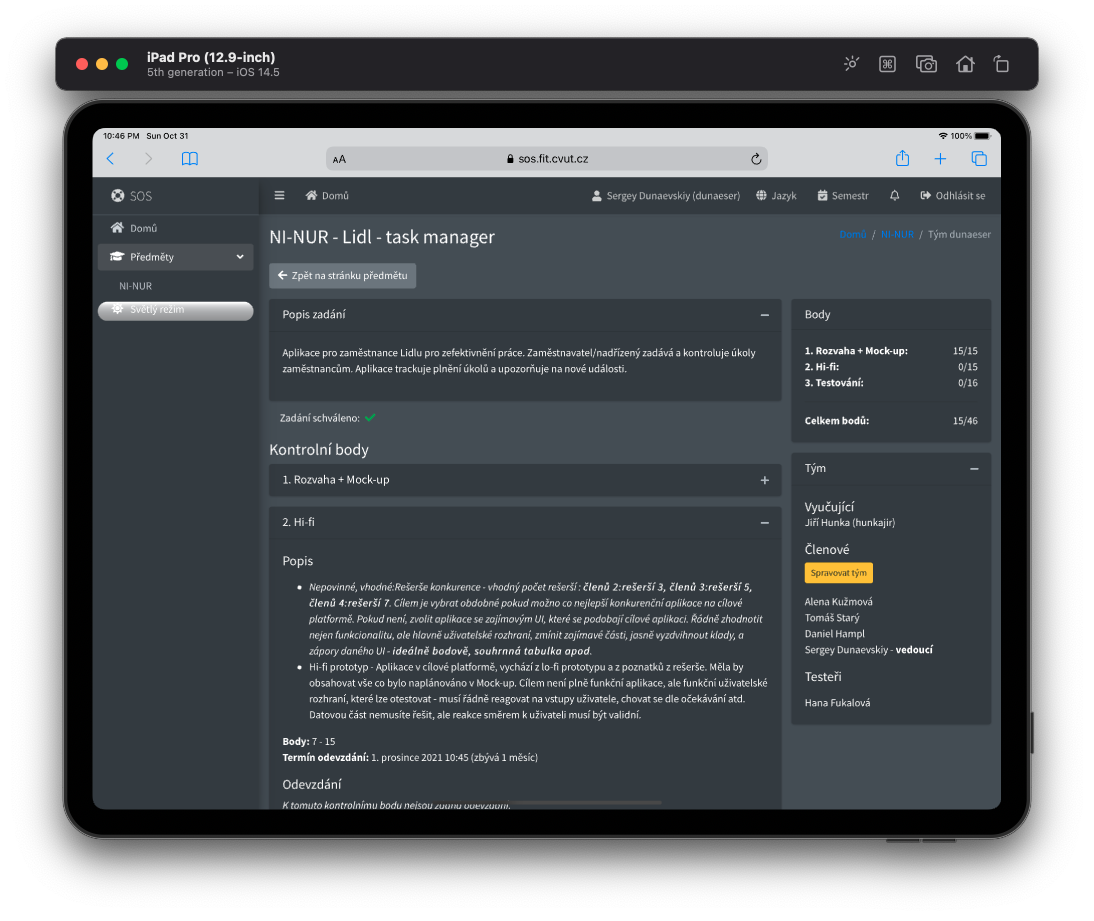
\includegraphics[max width=\textwidth]{assets/analysis-sos-portal}
   \caption[Studentský odevzdávací systém - ukázka detailu projektu]{Studentský odevzdávací systém - ukázka detailu projektu z pohledu studenta}\label{pic:sos-portal}
\end{figure}


Studentský odevzdávací systém je relativně nový portál -- nachází se v alpha verzi a využívá se například v předmětu NI-NUR\footnote{Návrh uživatelského rozhraní}.
Konceptuálně je myšlen jako univerzální systém pro všechny možné projekty, které vyžadují iterativní odevzdávání souborů a obdržení ohodnocení za odevzdanou práci.
Z pohledu studenta lze vytvořit návrhu projektu, který může, ale nemusí být schválen vyučujícím, bohužel nelze vytvářet nekontrolované projekty pro vlastní účely.
Následuje tvorba projektu mimo systém a odevzdávání výsledků v podobě samostatnách souborů s případným komentářem.
Započatý projekt nelze přerušit ze strany studenta.
Daný systém se v mnoha ohledech podobá \gls{IS}, který byl analyzován v předchozích kapitolách.

\textbf{Společné rysy}

\begin{ul}
   \item
   \textbf{Iterativní odevzdávání projektu} - založený projekt se odevzdává v iteracích (kontrolních bodech), které mohou být okomentovány a ohodnoceny ze strany vyučujícího.
   \item
   \textbf{Odpovědná osoba} - existuje role (vyučující), která dokáže ohodnotit kontrolní bod určitých počtem bodů.
\end{ul}


\textbf{Výhodné prvky}

\begin{ul}
   \item
   \textbf{Nahrávání souborů} - v rámci iterace lze nahrávat libovolné soubory.
   \item
   \textbf{Integrace s fakultními systémy} - \gls{IS} je víc přizpůsobený pro fakultní účely.
   \item
   \textbf{Tmavé rozhraní} - \gls{UI} má volitelný tmavý režim, viz obrázek~\ref{pic:sos-portal}.
   \item
   \textbf{Jazyky} - \gls{UI} je poskytováno v anglickém a českém jazyku s libovolným přepínáním.
\end{ul}


\textbf{Negativní prvky}

\begin{ul}
   \item
   \textbf{Restrikce zakládání projektů} - studenti nemohou zakládat vlastní, nezávislé projekty, musí spadat pod určitý předmět.
   Nelze založit a spravovat víc projektů.
   \item
   \textbf{Nelze založit víc projektových rolí} - projektové role i pro vedoucího projektu jsou omezeny na členy týmu a testery, nelze přidat libovolnou roli.
   \item
   \textbf{Neintuitivní rozhraní} - některé prvky uživatelského rozhraní nejsou intuitivně pochopitelné (subjektivně) a při kritické změně nevyžadují potvrzení.
\end{ul}
